\section{A Hybrid Compact Neural Architecture for Visual Place
Recognition}

\emph{IEEE ROBOTICS AND AUTOMATION LETTERS, VOL. 5, NO. 2, APRIL 2020}
{[}4{]}

\subsection{Introduction}\label{header-n182}

Performing visual place recognition (VPR) reliably is a challenge for
any robotic system or autonomous vehicle operating over long periods in
real-world environments. Convolutional neural networks (CNN) have been
applied to the field of VPR with great success, typically using
dedicated hardware: the GPUs. However, classical CNNs neglect any
temporal information between consecutive images. However, sequence-based
algorithms, such as SeqSLAM, matching two or more sequences of images to
perform VPR. Two main deep learning models can be used to capture
sequence patterns: \emph{computer-science-oriented} and
\emph{neuroscience-oriented} models. In recent researches, recurrent
neural networks (RNN) are used to reproduce the multi-scale spatial
representation of an environment. While the results are promising, these
computer-science-oriented systems are tested only in small synthetic
environments, and the integration with neuroscience-oriented recurrent
models such as continuous attractor neural networks (CANN) is not well
explored. An attractor network is a network of nodes (i.e. neurons),
often recurrently connected, whose time dynamics settle to a stable
pattern. A pattern can be stationary, time-varying (i.e. cyclic), or
chaotic. The particular pattern which network settles to is called its
\emph{attractor}. In neuroscience theory, different kinds of attractor
neural networks have been associated with different functions, such as
memory, motor behavior, and classification. More in detail, a continuous
attractor network is a special type of attractor network, which models a
non-linear dynamical system. A dynamical system consists of a
\emph{state place}, which its coordinates describe the state at any
instance and a \emph{dynamical role} that specifies the immediate future
of all state variables. For example, the state of a pendulum is its
angle and angular velocity, and the evolution rule is Newton's equation
\emph{F}=\emph{m\^{}a}. An \emph{attractor} can be discrete (a discrete
set of points) or continuous (a continuous object embedded in the state
space).

\begin{figure}[h!]
\centering
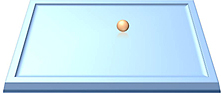
\includegraphics[width=0.5\linewidth]{images/continuousattractor.jpg}
\caption{A system (the yellow ball) with a continuous attractor (the blue surface)}
\end{figure}

In this work, the authors propose a hybrid neural network that
incorporates both computer-science- and neuroscience-oriented models to
perform the VPR task. Their approach comprises two key components:
FlyNet, a compact neural network, and a 1-d CANN as a temporal model
that encodes sequences of images to perform appearance-invariant VPR
using real data. The resulting FlyNet+CANN model achieves competitive
AUC results, but with far fewer parameters, minimal training time and
smaller computational footprint than conventional deep learning and
algorithmic-based approaches.

\begin{figure}[h!]
\centering
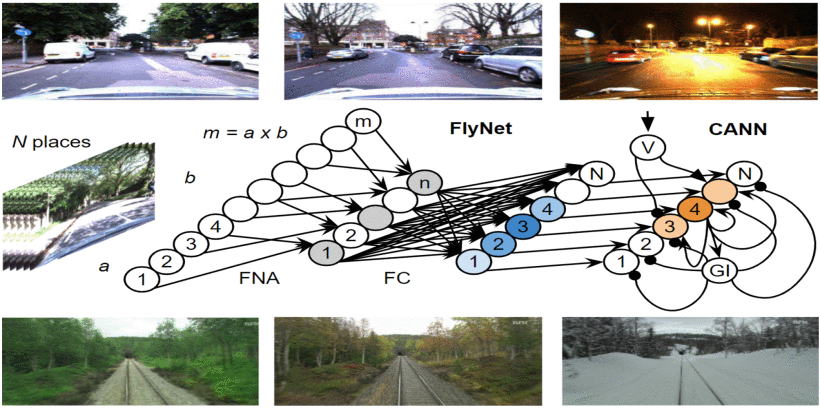
\includegraphics[width=0.8\linewidth]{images/flynetcann.png}
\caption{FlyNet+CANN hybrid neural architecture}
\end{figure}

\subsection{Previous work}\label{header-n187}

To design deep-learning-based models for VPR it is necessary to explore
how this activity is performed by mammalians' brains and take
inspiration from it. RatSLAM is an example, this method performs visual
SLAM implementing the mechanisms using by rodents' brain. Other models
perform VPR following the insect brains, like ants, bees, and flies,
that exhibits the great capacity to navigate. Place recognition in
insects is, however, most likely mediated by processing within the
\emph{mushroom bodies} (MB), a pair of structures involved in
classification, learning, and recognition of both olfactory and visual
information. Their structure has been similar to a multi-layer
perceptron (MLP) network, which receives massive input signals from
sensory lobes. These impressive capabilities, achieved with relatively
small brains, make them attractive models for roboticists. For FlyNet,
we take inspiration from algorithmic insights found in the fruit fly
olfactory neural circuit. The authors investigate how it can be
integrated with recurrent-based networks for the VPR task. Classical CNN
models for image recognition have good performance but they have also
undesirable characteristics. In fact, these networks are difficult to
implement in a real robot, due to their size and complexity. In
contrast, the authors propose the usage of compact neural models such as
FlyNet to alleviate these requirements. To access and exploit the power
of temporal information in many applications, researchers have developed
a range of RNN. Another approach, implementing by RatSLAM, uses
incorporated multi-dimensional CANN models with pre-assigned weights and
structure. There exist other non-neural techniques, like SeqSLAM, that
match sequences of pre-processed frames to provide an estimate of place.
In this work, the authors attempt to develop a new bio-inspired, hybrid
neural network for VPR tasks based on insect brain architectures such as
FlyNet, which is extremely compact and can incorporate the filtering
capabilities of a 1-d CANN to achieve competitive localization results.

\subsection{Proposed method}\label{header-n189}

\subsubsection{FlyNet algorithm}\label{header-n190}

The FlyNet proposed in this works is inspired by the \emph{fly
algorithm}. The Drosophila's small brain identifies odors by assigning
similar neural activity patterns to similar input odors. The neural
networks are composed of 4 layers (the input layer, two hidden layers,
and the output layer). The network works as follows. A binary, sparse
random matrix (\emph{random projection}) connects the input layer to the
second layer: each neuron receives and sums about 10\% of the input
neurons. This mechanism is also used to connect the second and third
layers, but the number of neurons in the third layer is the same as the
output one. Finally, using a WTA (winner-take-all) circuit, the third
layer's neurons are mapped to the output layer, setting the first 5\%
with the high value to 1 and the rest to 0. The input layer generates a
specific binary identifier for the input odor. The \emph{FlyNet
Algorithm} (FNA) proposed in this work is a mapping of the fly algorithm
for vision purposes. The only difference is the WTA circuit, which is
set to consider true the first 50\% of the neurons with the high
neurons.

\begin{figure}[h!]
\centering
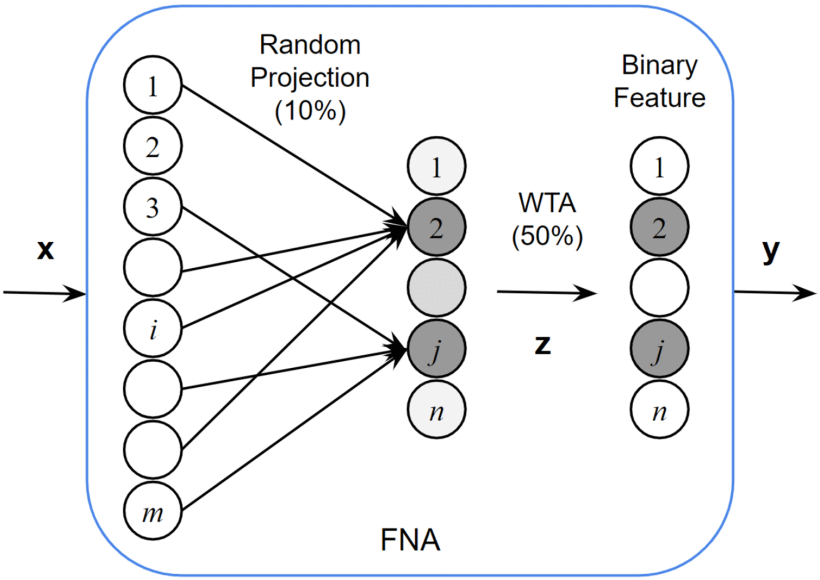
\includegraphics[width=0.7\linewidth]{images/fly.png}
\caption{The fly algorithm's network architecture. The random projection is shown only for the connection between the two hidden layer, but all the input layer is connected to the first hidden layer using the same mechanism}
\end{figure}

\subsubsection{FlyNet models}\label{header-n193}

The authors implement a range of VPR models, using FNA and a module with
temporal filtering capabilities. These networks models are the
following:

\begin{itemize}
\item
  \textbf{FlyNet:} it's composed by the FNA that terminates with a fully
  connected (FC) network. Its architecture is a three-layer MLP with
  64--64--1000 units respectively, where the first two layers make up
  the FNA and the last one composes the FC network.
\item
  \textbf{FlyNet+SeqSLAM:} it incorporates the SeqSLAM algorithm on top
  of our single-frame FlyNet network. This model can be compared along
  with the other following temporal models.
\item
  \textbf{FlyNet+RNN:} It is a purely neural model that incorporates an
  RNN on top of FlyNet and terminates with another FC layer. Its
  architecture is the same as FlyNet (the FC layers have 100 units),
  with 512 recurrent units. 
\item
  \textbf{FlyNet+CANN:} it incorporates a variation of the CANN
  architecture proposed in RatSLAM, which is a 1-dimensional model, on
  top of the FlyNet network. The CANN layer has 1002 units.
\end{itemize}

\begin{figure}[h!]
\centering
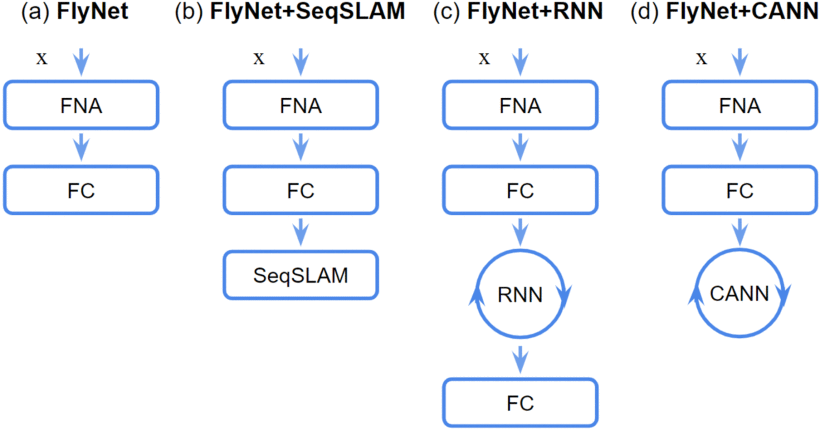
\includegraphics[width=0.8\linewidth]{images/flynetmodels.png}
\caption{FlyNet models}
\end{figure}

\subsection{Experiments}\label{header-n205}

\subsubsection{Dataset and data preprocessing}\label{header-n206}

To evaluate the capabilities of the proposed FlyNet-based models, the
authors conduct extensive experiments on two of the most widespread
benchmarks used in VPR, the \emph{Nordland} and \emph{Oxford RobotCar}
datasets. Nordland includes extreme seasonal changes across spring,
summer, fall, and winter, captured during a train journey, in northern
Norway. The summer traversal is used for training, and the remaining for
testing. The Oxford RobotCar dataset provides over 100 traverses with
different lighting (e.g. day, night) and weather (e.g. direct sun,
overcast) conditions through a car ride in Oxford city. The images are
pre-processed before being used by the models. FlyNet baselines convert
the images into single-channel (gray-scale) frames normalized between
{[}0, 1{]}, and then resize them to $32 \times 64$.

\subsubsection{Experiments evaluation}\label{header-n208}

The authors train and test the four FlyNet models in order to find the
best model and compare it with other existing state-of-the-art
techniques. In particular, these methods are \emph{SeqSLAM} (without FNA
attacked), \emph{LoST-X}, and \emph{Multi-Process Fusion}.

\paragraph{Metrics}\label{header-n210}

VPR models' performance is evaluated using precision-recall (PR) curves
and area under the curve (AUC) metrics. The tolerance used to consider a
query place as a correct match is being within 20 frames around the
ground truth location for the Nordland dataset, and up to 50 meters (10
frames) away from the ground truth for the Oxford RobotCar dataset.

\paragraph{Comparison of FlyNet to Other Neural
Networks}\label{header-n212}

FlyNet (alone) is compared with the other four single-frame models: a
simple FC network, an FC network with dropout, a CNN, and an
implementation of the NetVLAD method. The FC network has the same
architecture as FlyNet: it is a three-layer MLP with 64-64-1000 neurons
respectively. The FC network with dropout is the same as the previous
one, but with a dropout rate of 90\% and 50\% for the first and second
layers, respectively, in order to approximate the FlyNet sparsity and
for fair comparison purposes. The CNN model has 2 convolutional layers
while the NetVLAD output representation dimensionality is reduced from
4096 to 64 to be comparable in size with the FlyNet.
\newpage
\subsection{Experiments results}\label{header-n214}

\subsubsection{FlyNet vs. Other Single-Frame
Networks}\label{header-n215}

FlyNet is directly competitive with both FC networks, despite FlyNet
having over 3 times fewer parameters (64 k vs. 199 k). CNN and NetVLAD
models, with 6 and 234 times more parameters than FlyNet respectively,
the larger the model the better the results we obtained. Under
\emph{small environmental changes} (e.g. summer to fall) both networks
achieved over 70\% AUC. However, under \emph{extreme visual changes}
(e.g. summer to winter) all these models show relatively similar
results, below 12\% AUC, except for NetVLAD with 20\% AUC.

\begin{figure}[h!]
\centering
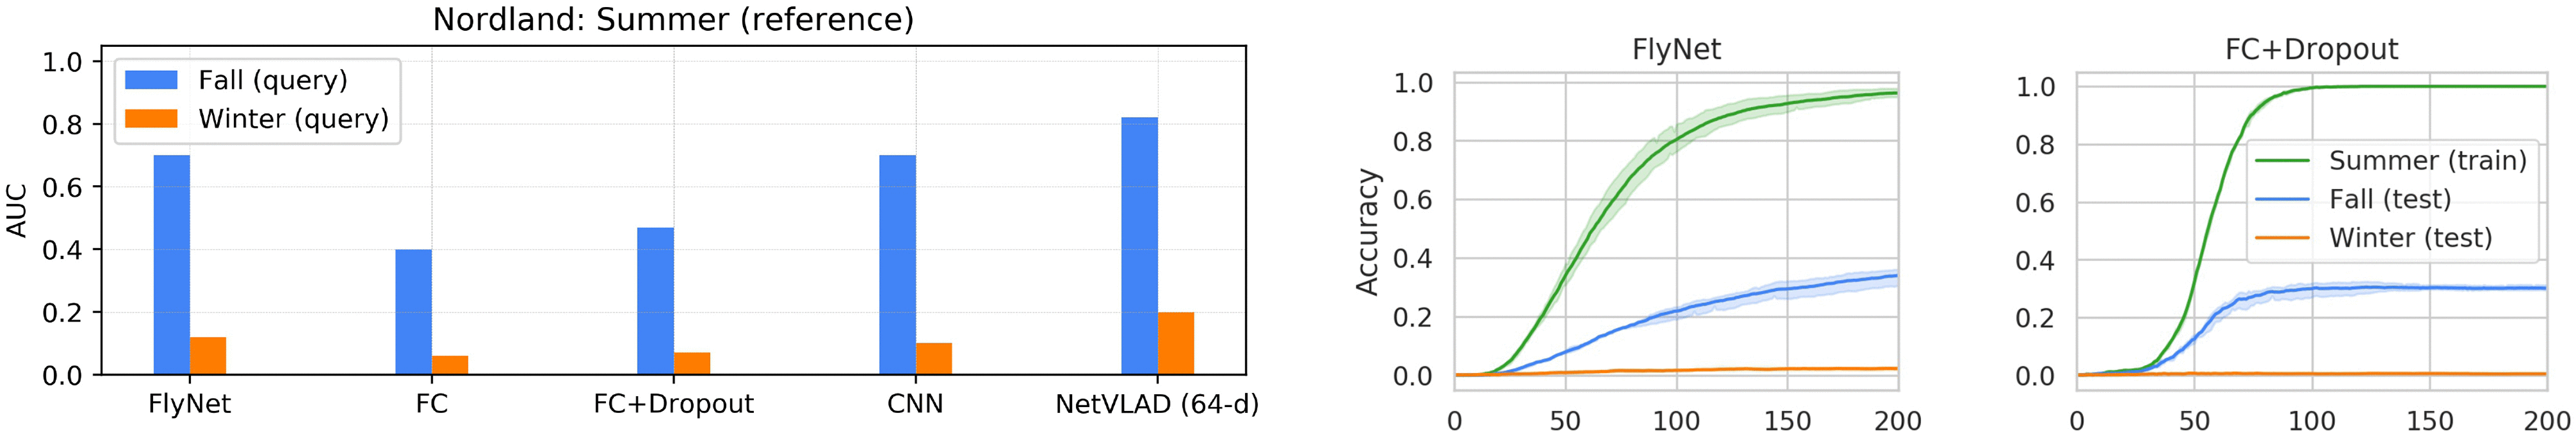
\includegraphics[width=\linewidth]{images/flynetothermodels.png}
\caption{Comparison of FlyNet (alone) to other single-frame neural networks. AUC results across different models on the Nordland dataset (left). Average accuracy over 10 training experiments vs. number of epochs for FlyNet (middle) and a fully connected (FC) network with dropout (right).}
\end{figure}

\subsubsection{FlyNet models evaluation}\label{header-n218}

Although there are significant performance differences at a single-frame
matching level, the figure below shows that when using sequence-based
filtering techniques these differences reduce significantly. For
FlyNet+SeqSLAM, the performance of FlyNet (alone) was significantly
improved. Similarly, the RNN layer on top of FlyNet improved even
further these results. However, when integrating the output of FlyNet
with a 1-d CANN we were able to outperform these models, even under
extreme environmental changes: this is the best model.

\begin{figure}[h!]
\centering
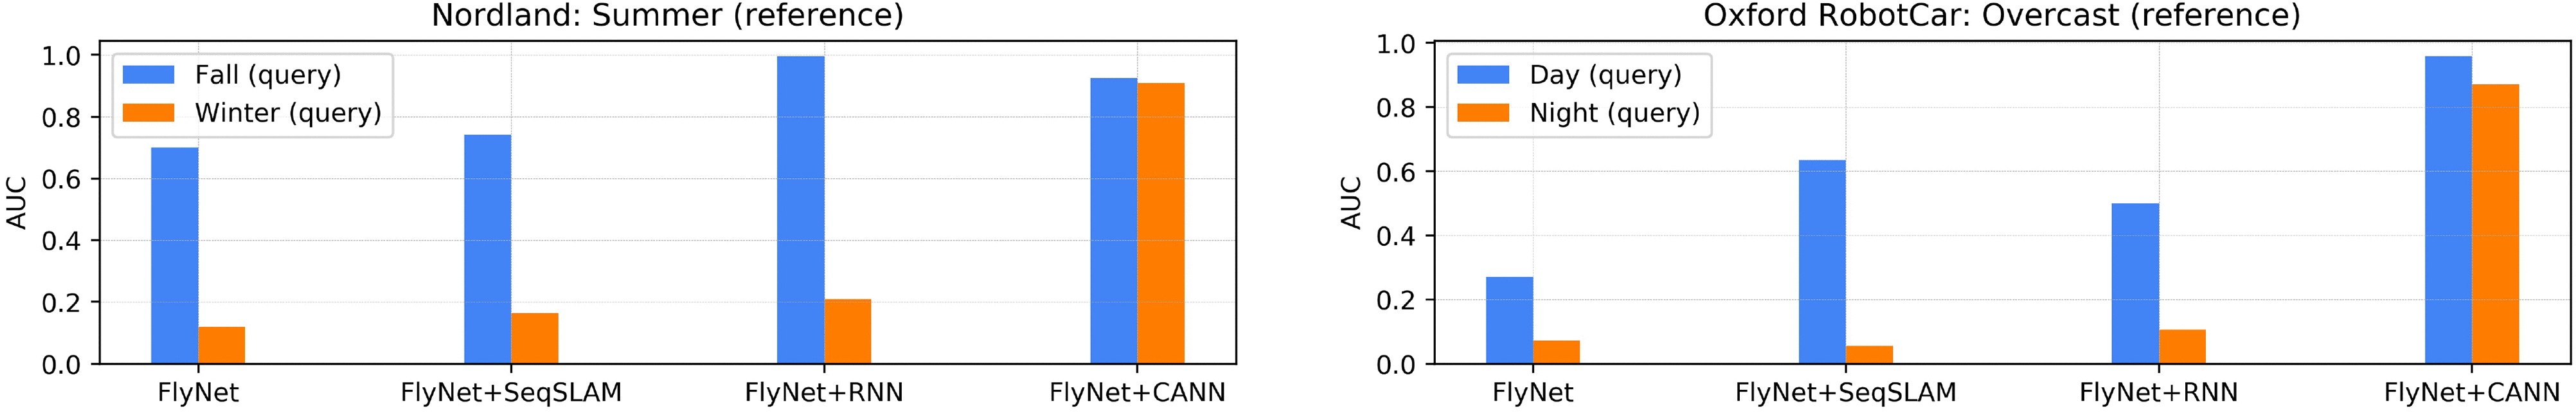
\includegraphics[width=1\linewidth]{images/flynetcomparemodels.png}
\caption{AUC results of the four FlyNet models}
\end{figure}

\newpage

\subsubsection{Best model vs. state-of-the-art
methods}\label{header-n221}

MPF is performing better while being able to recall almost all places at
100\% precision on both fall and winter testing traverses. FlyNet+CANN
achieves state-of-the-art results, comparable with SeqSLAM and MPF in
all these tested traverses.

\begin{figure}[h!]
\centering
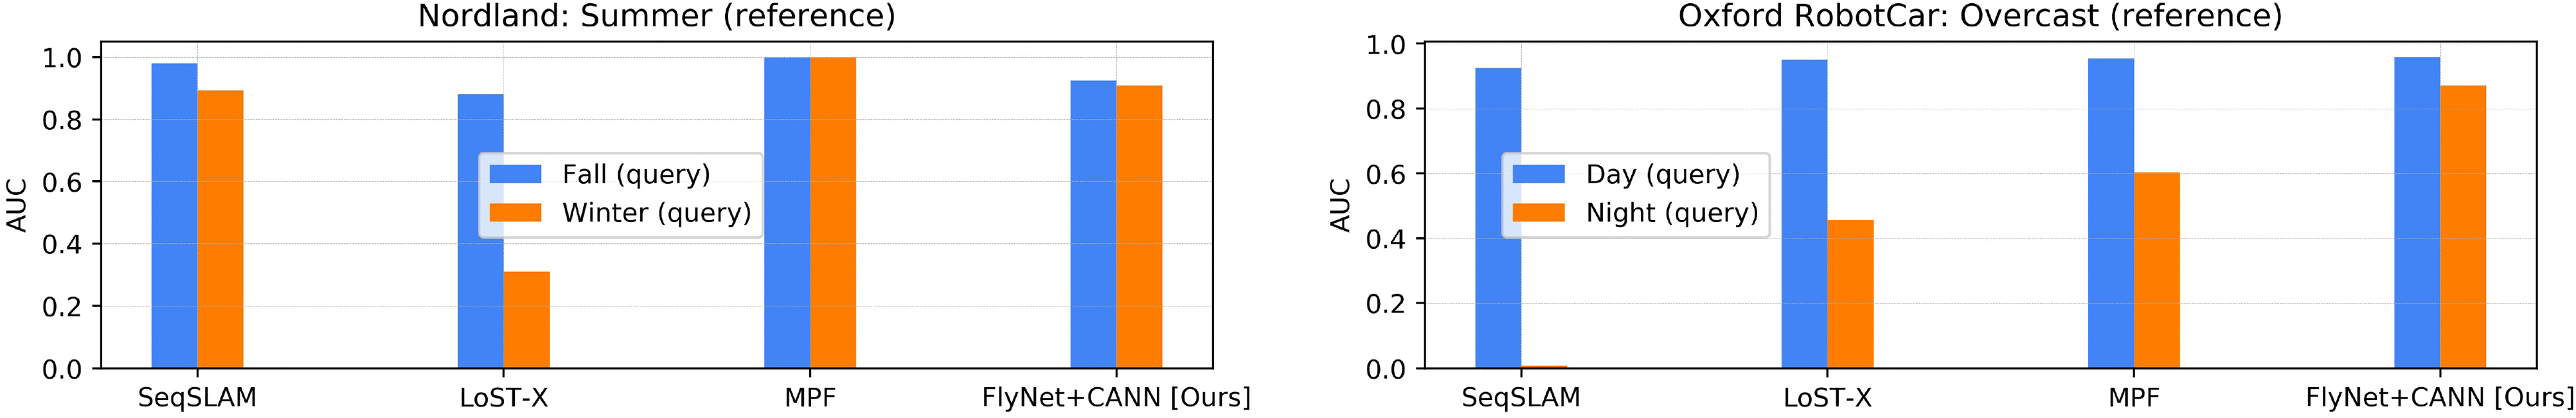
\includegraphics[width=1\linewidth]{images/bestmodelvsothers.png}
\caption{AUC results of the state-of-the-art methods measured on the two dataset}
\end{figure}

Similarly, PR performance on the Oxford RobotCar dataset is shown in the
following figure. FlyNet+CANN not only achieves state-of-the-art results
comparable with the other methods, but it maintains PR performance even
under extreme environmental changes (e.g. overcast to night), as shown
the bottom-right side of the figure.

\begin{figure}[h!]
\centering
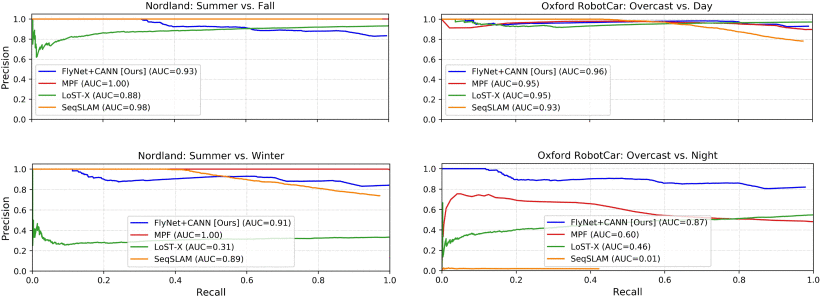
\includegraphics[width=1\linewidth]{images/bestmodelvsothersPR.png}
\caption{PR results of the state-of-the-art methods measured on the two dataset}
\end{figure}

\subsubsection{Computational performance}\label{header-n226}

The processing time required to perform appearance-invariant VPR by our
hybrid model is compared to those from state-of-the-art methods in terms
of running time for (1) feature extraction, (2) visual place matching
between query and reference traverses, and (3) average place recognition
time for a single query image from a 1000-image reference database. This
Avg. Time (3) is calculated as (Feature Ext. (1) + Place Match.
(2))/1000. Processing time results on the Nordland dataset are reported
in the following table. The FlyNet+CANN can be up to 6.5, 310, and 1.5
times faster than MPF, LoST-X, and SeqSLAM, respectively.

\begin{longtable}[]{@{}llll@{}}
\toprule
\textbf{Method} & \textbf{Feature extraction} & \textbf{Place matching}
& \textbf{Avg. time (fps)}\tabularnewline
\midrule
\endhead
\textbf{FlyNet+CANN} & \textbf{35 sec} & \textbf{25 sec} & \textbf{0.06
sec (16.66)}\tabularnewline
MPF & 1.9 min & 4.6 min & 0.39 sec (2.56)\tabularnewline
LoST-X & 110 min & 200 min & 18.6 sec (0.05)\tabularnewline
SeqSLAM & 50 sec & 40 sec & 0.09 sec (11.11)\tabularnewline
\bottomrule
\caption{Processing time comparison on the Nordland dataset}
\end{longtable}

The following figure shows the comparison between the networks'
complexity and the results obtained, viewing the AUC metric for the most
challenging appearance change (day to night). The best model proposed in
this works obtains the best results with the minimum number of
parameters.

\begin{figure}[h!]
\centering
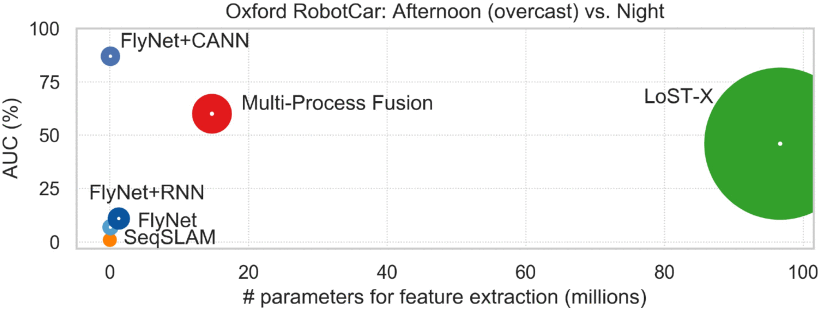
\includegraphics[width=1\linewidth]{images/flynetothermodeldimensions.png}
\caption{Oxford RobotCar AUC performance vs. Network Size. Comparison for the most challenging appearance change (day to night)}
\end{figure}

\subsection{Conclusions}\label{header-n256}

FlyNet+CANN model achieves competitive visual localization results
compared to existing deep learning and algorithmic-based VPR techniques,
but with significantly fewer parameters, a smaller footprint, and
reduced processing time. The authors want to demonstrate that, taking
inspiration from the biological brain, it is possible to build
sample-efficient, high-performing VPR models. FlyNet has the same number
of layers and sparse structure found in the fly olfactory neural
circuit. Despite the fly, brains extend by forty times the
dimensionality of the inputs, the authors have experimentally shown that
also reducing this dimension the FlyNet training accuracy remained
around 96\%. At the same time, FlyNet+CANN enabled the use of a
relatively low-performance but fast network to get better VPR results,
which is also able to generalize across challenging environmental
changes.